% Options for packages loaded elsewhere
\PassOptionsToPackage{unicode}{hyperref}
\PassOptionsToPackage{hyphens}{url}
%
\documentclass[
  ignorenonframetext,
]{beamer}
\usepackage{pgfpages}
\setbeamertemplate{caption}[numbered]
\setbeamertemplate{caption label separator}{: }
\setbeamercolor{caption name}{fg=normal text.fg}
\beamertemplatenavigationsymbolsempty
% Prevent slide breaks in the middle of a paragraph
\widowpenalties 1 10000
\raggedbottom
\setbeamertemplate{part page}{
  \centering
  \begin{beamercolorbox}[sep=16pt,center]{part title}
    \usebeamerfont{part title}\insertpart\par
  \end{beamercolorbox}
}
\setbeamertemplate{section page}{
  \centering
  \begin{beamercolorbox}[sep=12pt,center]{part title}
    \usebeamerfont{section title}\insertsection\par
  \end{beamercolorbox}
}
\setbeamertemplate{subsection page}{
  \centering
  \begin{beamercolorbox}[sep=8pt,center]{part title}
    \usebeamerfont{subsection title}\insertsubsection\par
  \end{beamercolorbox}
}
\AtBeginPart{
  \frame{\partpage}
}
\AtBeginSection{
  \ifbibliography
  \else
    \frame{\sectionpage}
  \fi
}
\AtBeginSubsection{
  \frame{\subsectionpage}
}
\usepackage{amsmath,amssymb}
\usepackage{iftex}
\ifPDFTeX
  \usepackage[T1]{fontenc}
  \usepackage[utf8]{inputenc}
  \usepackage{textcomp} % provide euro and other symbols
\else % if luatex or xetex
  \usepackage{unicode-math} % this also loads fontspec
  \defaultfontfeatures{Scale=MatchLowercase}
  \defaultfontfeatures[\rmfamily]{Ligatures=TeX,Scale=1}
\fi
\usepackage{lmodern}
\ifPDFTeX\else
  % xetex/luatex font selection
\fi
% Use upquote if available, for straight quotes in verbatim environments
\IfFileExists{upquote.sty}{\usepackage{upquote}}{}
\IfFileExists{microtype.sty}{% use microtype if available
  \usepackage[]{microtype}
  \UseMicrotypeSet[protrusion]{basicmath} % disable protrusion for tt fonts
}{}
\makeatletter
\@ifundefined{KOMAClassName}{% if non-KOMA class
  \IfFileExists{parskip.sty}{%
    \usepackage{parskip}
  }{% else
    \setlength{\parindent}{0pt}
    \setlength{\parskip}{6pt plus 2pt minus 1pt}}
}{% if KOMA class
  \KOMAoptions{parskip=half}}
\makeatother
\usepackage{xcolor}
\newif\ifbibliography
\usepackage{graphicx}
\makeatletter
\def\maxwidth{\ifdim\Gin@nat@width>\linewidth\linewidth\else\Gin@nat@width\fi}
\def\maxheight{\ifdim\Gin@nat@height>\textheight\textheight\else\Gin@nat@height\fi}
\makeatother
% Scale images if necessary, so that they will not overflow the page
% margins by default, and it is still possible to overwrite the defaults
% using explicit options in \includegraphics[width, height, ...]{../figures/}
\setkeys{Gin}{width=\maxwidth,height=\maxheight,keepaspectratio}
% Set default figure placement to htbp
\makeatletter
\def\fps@figure{htbp}
\makeatother
\setlength{\emergencystretch}{3em} % prevent overfull lines
\providecommand{\tightlist}{%
  \setlength{\itemsep}{0pt}\setlength{\parskip}{0pt}}
\setcounter{secnumdepth}{-\maxdimen} % remove section numbering
% Slide layout defaults for warning-clean scientific decks.
\usepackage{etoolbox}
\IfFileExists{xurl.sty}{\usepackage{xurl}}{}
\IfFileExists{seqsplit.sty}{\usepackage{seqsplit}}{\newcommand{\seqsplit}[1]{#1}}
\protected\def\breakseq#1{\seqsplit{#1}}
\protected\def\breaktt#1{\begingroup\ttfamily\seqsplit{#1}\endgroup}
\setlength{\emergencystretch}{6em}
\tolerance=5000
\hbadness=10000
\hfuzz=1pt
\setlength{\tabcolsep}{2pt}
\AtBeginEnvironment{longtable}{\tiny\renewcommand{\arraystretch}{0.86}\setlength{\tabcolsep}{1pt}}
\AtBeginEnvironment{tabular}{\tiny\renewcommand{\arraystretch}{0.86}\setlength{\tabcolsep}{1pt}}

% Natbib and cross-reference fallbacks — slides don't load natbib
% or cleveref, but combined-PDF manuscript prose may emit these
% commands. The fallback renders citations as a bracketed key list
% and cross-references as detokenized labels so slides don't fail on
% undefined control sequences or raw underscores. \providecommand is
% a no-op if packages load later.
\providecommand{\citep}[1]{[#1]}
\providecommand{\citet}[1]{#1}
\providecommand{\citealp}[1]{#1}
\providecommand{\citeauthor}[1]{#1}
\providecommand{\citeyear}[1]{#1}
\providecommand{\cref}[1]{\texttt{\detokenize{#1}}}
\providecommand{\Cref}[1]{\texttt{\detokenize{#1}}}

\newtheorem{proposition}{Proposition}
\newtheorem{hypothesis}{Hypothesis}
\ifLuaTeX
  \usepackage{selnolig}  % disable illegal ligatures
\fi
\usepackage{bookmark}
\IfFileExists{xurl.sty}{\usepackage{xurl}}{} % add URL line breaks if available
\urlstyle{same}
\hypersetup{
  hidelinks,
  pdfcreator={LaTeX via pandoc}}

\author{}
\date{}

\begin{document}

\section{Results: Citation Network}\label{results-citation-network}

\begin{frame}[allowframebreaks]{RQ4: Citation Geometry}
\phantomsection\label{rq4-citation-geometry}
Resolving each record's references against the corpus yields an
intra-corpus citation graph (built and analyzed with NetworkX
\breakseq{[@hagberg2008exploring]}) of \{\{CITATION\_NODES\}\} nodes and
\{\{CITATION\_EDGES\}\} edges across \{\{CITATION\_COMPONENTS\}\}
connected components, with a graph density of
\{\{CITATION\_DENSITY\_PCT\}\}\% and a mean in-degree of
\{\{MEAN\_IN\_DEGREE\}\}. Of \{\{CITATION\_TOTAL\_REFS\}\} total
outgoing references, \{\{CITATION\_RESOLUTION\_PCT\}\}\% resolve to
another record inside the corpus. This resolution rate describes how
self-contained the retrieved slice is; it is not an estimate of the
underlying citation density of any individual work.

The citation network has \{\{CITATION\_COMMUNITIES\}\} communities
(detected by modularity optimization), a maximum in-degree of
\{\{CITATION\_MAX\_IN\_DEGREE\}\} (the most-cited paper within the
corpus), and a maximum out-degree of \{\{CITATION\_MAX\_OUT\_DEGREE\}\}
(the paper that cites the most other corpus members).
\end{frame}

\begin{frame}[allowframebreaks]{Centrality Analysis}
\phantomsection\label{centrality-analysis}
Centrality scores (PageRank \breakseq{[@page1999pagerank]} and HITS) and
modularity-based community detection \breakseq{[@clauset2004finding]} are
rounded and ranked with a stable tiebreaker so the reported hub and
authority rankings are byte-reproducible across runs despite the
floating-point non-associativity of the underlying iterative solvers.

\textbf{Table 4. Top 5 papers by PageRank.}

\{\{TOP\_PAGERANK\_TABLE\}\}

\textbf{Table 5. Top 5 authority papers (HITS).}

\{\{TOP\_AUTHORITIES\_TABLE\}\}

\textbf{Table 6. Top 5 hub papers (HITS).}

\{\{TOP\_HUBS\_TABLE\}\}

The highest-ranked paper by PageRank (DOI \{\{TOP\_PAGERANK\_DOI\}\}) is
a central node in the retained citation graph. Its score indicates
relative centrality within this graph, not scientific importance or
causal influence. Hub papers cite many corpus members and may connect
threads of the retrieved literature, but their role should be checked
against their source type and content.

\begin{figure}
\centering
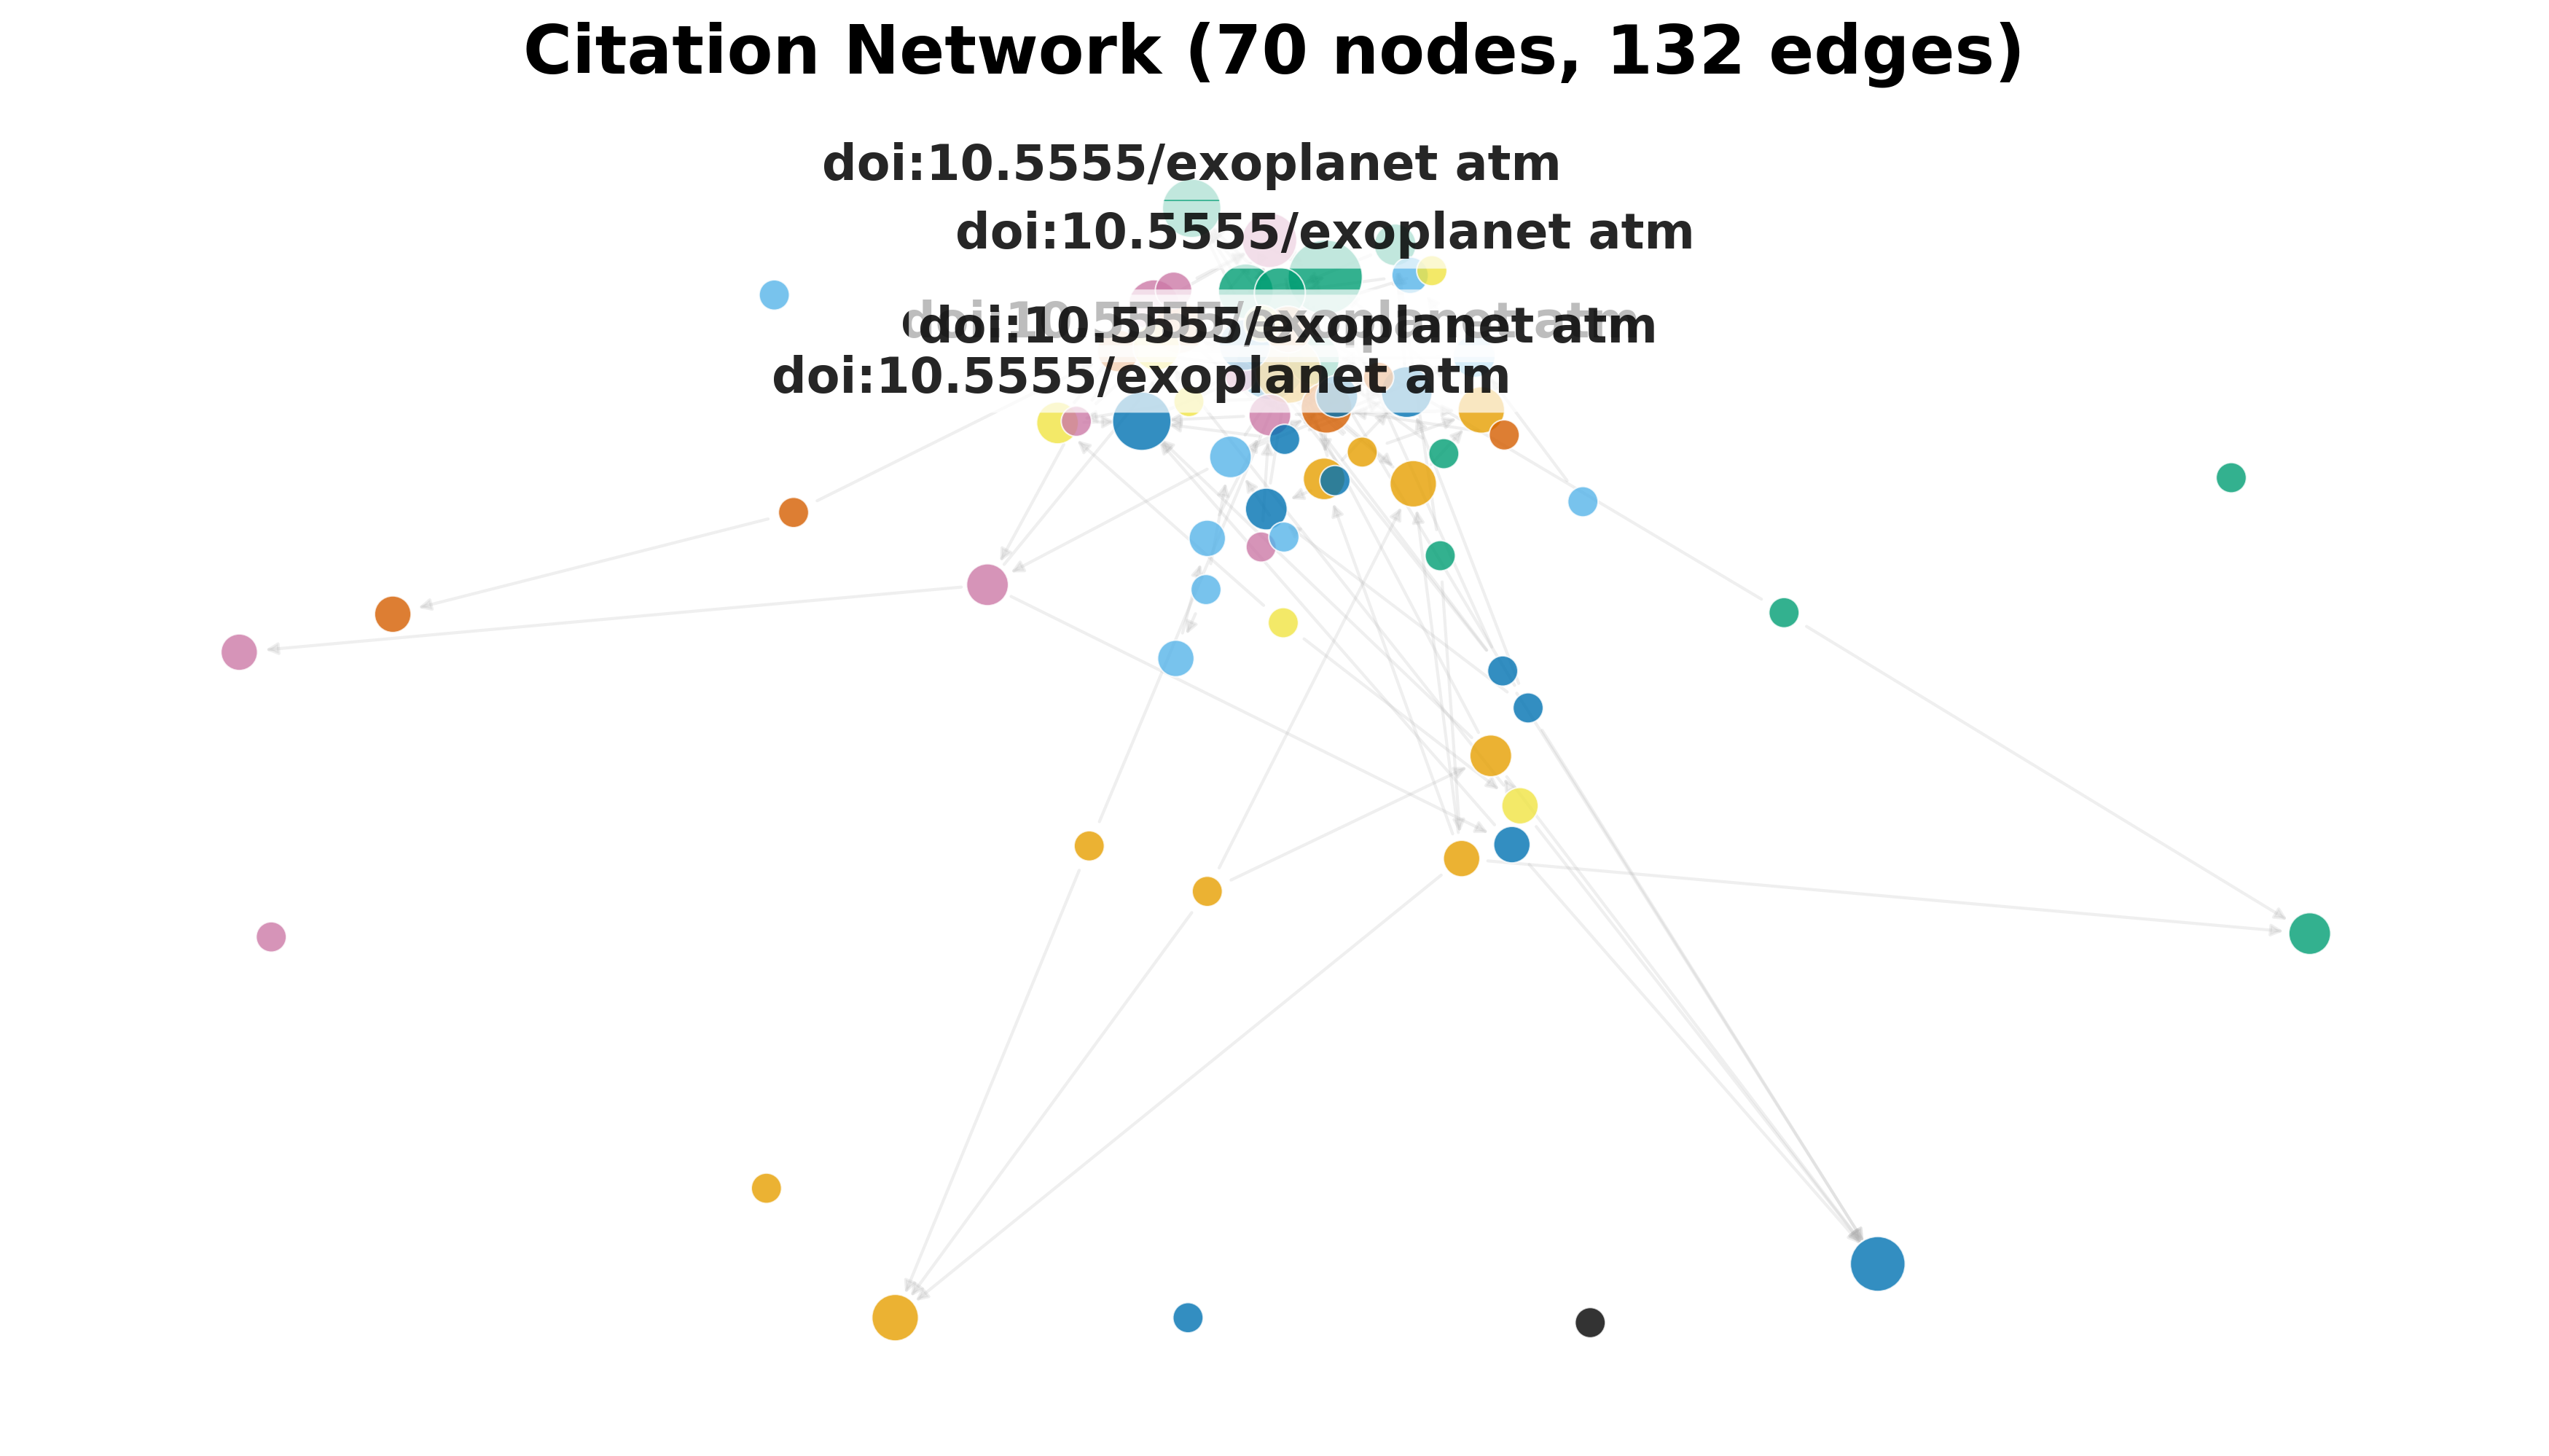
\includegraphics{../figures/citation_network.png}
\caption{Citation network for \{\{SEARCH\_TERM\_TITLE\}\}. Nodes
represent papers; directed edges represent citation links. Node colours
indicate community membership (\{\{CITATION\_COMMUNITIES\}\} communities
detected by modularity optimization). Layout uses a spring-based
algorithm with a fixed seed for
reproducibility.}\label{fig:citation_network}
\end{figure}

\begin{figure}
\centering
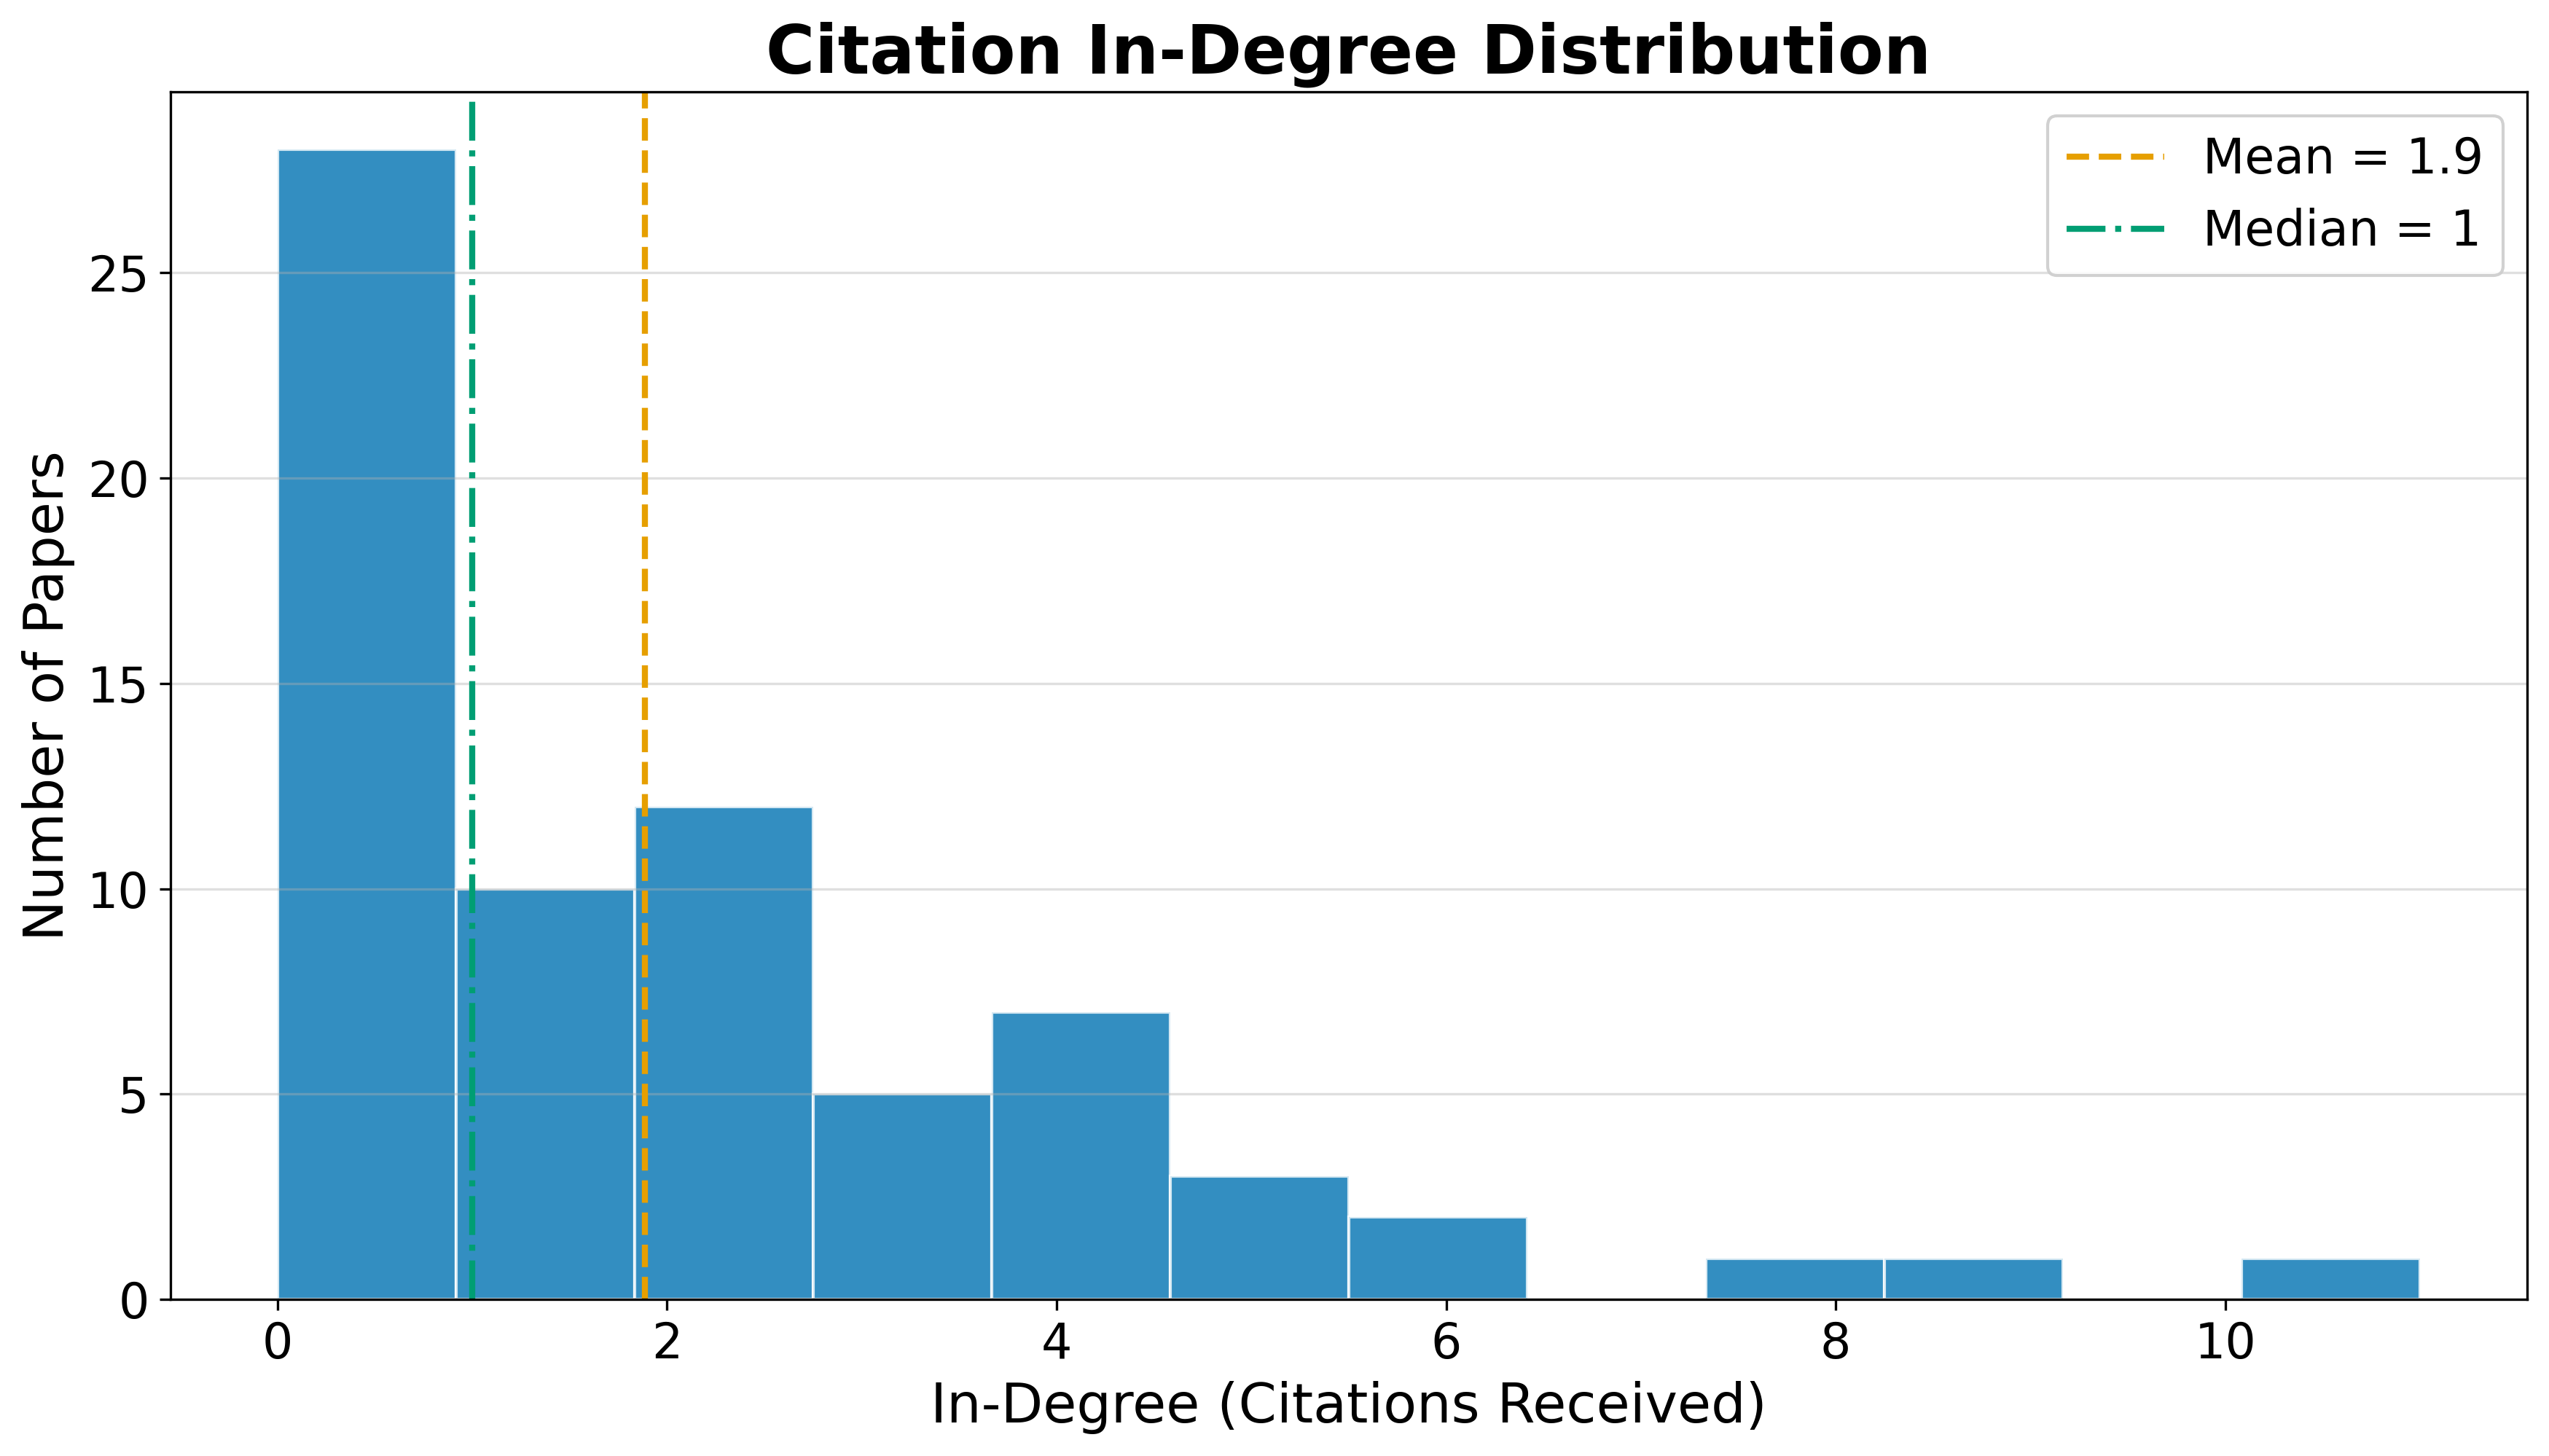
\includegraphics{../figures/degree_distribution.png}
\caption{Degree distribution for the \{\{SEARCH\_TERM\_TITLE\}\}
citation network. The histogram shows the frequency of each in-degree
value on a log-linear scale, revealing the heavy-tailed structure
characteristic of citation networks.}\label{fig:degree_distribution}
\end{figure}

The heavy-tailed degree distribution is characteristic of citation
networks: a small number of highly-cited papers anchor the structure,
while the long tail of low-degree nodes represents newer or peripheral
works. The low graph density (\{\{CITATION\_DENSITY\_PCT\}\}\%) reflects
the sparsity of intra-corpus citation links. Many papers may cite works
outside the retrieved slice, especially under a capped retrieval design.
\end{frame}

\begin{frame}[allowframebreaks]{Advanced Network Metrics}
\phantomsection\label{advanced-network-metrics}
Beyond PageRank and HITS, the network analysis computes betweenness
centrality (which papers bridge different communities), closeness
centrality (which papers are near all others), degree assortativity (do
highly-cited papers cite other highly-cited papers?), and average
clustering coefficient (how tightly knit are local neighborhoods).

The degree assortativity coefficient is \{\{DEGREE\_ASSORTATIVITY\}\},
and the average clustering coefficient is \{\{AVG\_CLUSTERING\}\}. A
negative assortativity indicates that highly-cited papers tend to cite
less-cited papers (dissortative mixing), which is typical of citation
networks where review papers (high in-degree) cite many primary studies
(low in-degree).

\textbf{Table 7. Top 5 papers by betweenness centrality.}

\{\{TOP\_BETWEENNESS\_TABLE\}\}

Papers with high betweenness centrality occupy shortest paths between
communities in the retained graph. Removing one may alter connectivity,
but that graph operation does not by itself establish that the paper is
a review or methodological bridge in the scientific field. Source-type
and content review are required for that interpretation.
\end{frame}

\end{document}
